\documentclass[12pt,a4paper]{article}
\usepackage[utf8]{inputenc}
\usepackage[dvips]{graphicx}
\usepackage[russian]{babel}
\usepackage[colorlinks,urlcolor=blue,citecolor=blue,linkcolor=black,menucolor=black]{hyperref}
\usepackage{color}
\usepackage{cite}
\usepackage{bm}
\usepackage{cmap}
\usepackage{indentfirst}
\usepackage{amssymb}
\usepackage{amsmath}  
\usepackage{tabularx}

\setcounter{tocdepth}{2}
\begin{document}
	\begin{titlepage}
		\begin{center}
			Федеральное государственное бюджетное образовательное учереждение\\
			высшего образования\\[0.5cm]
			Омский государственный университет им. Ф.М. Достоевского\\[0.5cm]
			Кафедра теоритической физики\\[2cm]
			
			Отчет о выполнении учебного задания №1 по <<Вычислительной физике>>\\
			
			{\large{Исследование статистических характеристик ГПСЧ, входящих в стандартную библиотеку C++  }}\\[2cm]
		\end{center}
		
		\begin{flushright}
			Выполнил:\\ студент группы ФПБ - 603\\
			Ватолкин Михаил Александрович\\[2cm]
			Проверил:\\
			Попов И.С.\\[2cm]
			Заведующий кафедрой:\\
			доктор физ.-мат. наук,\\
			профессор Прудников В.В.\\*[2cm]
		\end{flushright}
		
		\begin{center}
			Омск--2018
		\end{center}
	\end{titlepage}
	\newpage
	
	\setcounter{page}{2} \tableofcontents
	\newpage
	\graphicspath{{pic/}}
	\DeclareGraphicsExtensions{.eps}
		\section*{Введение}
	В данной работе исследование проводилось для решеток с линейными размерами 128, 256, 512, в температурном диапазоне $T \in[1.8, 2.8]$.
	Было исследовано поведение восприимчивости, кумулянты Биндера и намагниченности.
	Поиск критической точки осуществлялся наложением графиков зависимости кумулянты Биндера от времени.
	Так же прилагается исследование времени расчетов для разных систем на разных разных ЭВМ.
	\section{Намагниченность}
	Вблизи критической точки мы можем наблюдать резкое падение намагниченности, причем как мы можем видеть из графика, с ростом системы намагниченность стремится принять значение 0 в этой точке.
	\begin{center}
	\mbox{
		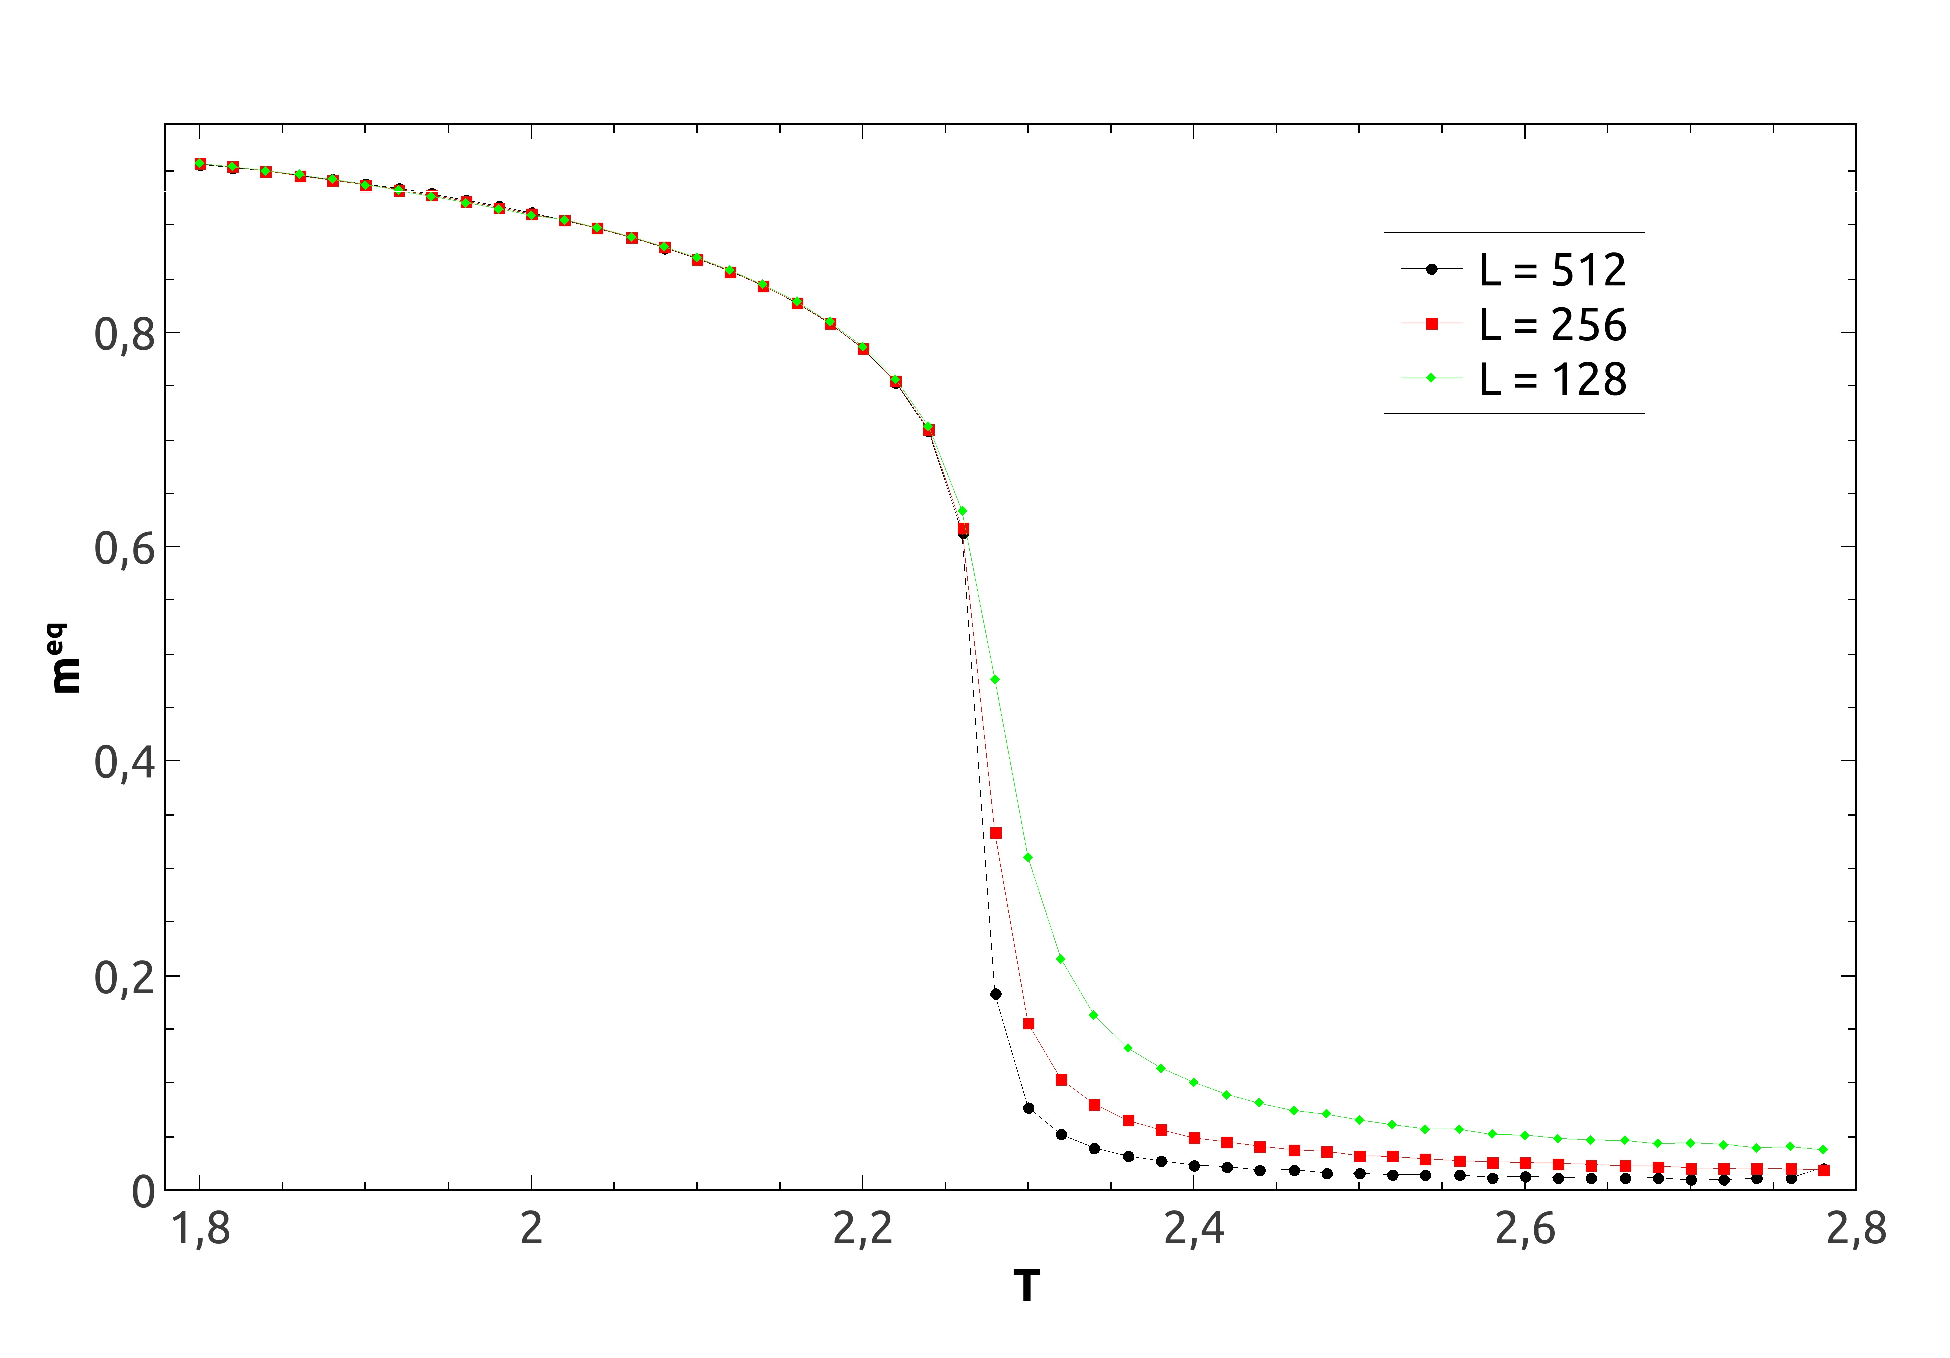
\includegraphics[scale=0.4]{meq}
	} 
	\end{center}
	\section{Восприимчивость}
	Здесь мы видим , что восприимчивость имеет пик, но он не совпадает с критической точкой, т.к он для систем с разными размерами принимает свое значение, но мы можем заметить, что с ростом системы он стремится к конкретной точки на оси $T$ и к бесконечности по оси $\chi$, такое поведение связано с конечно-разностными эффектами, обусловленными ограниченными размерами системы, что приводит к зависимости характеристик системы от ее размеров.
	\begin{center}
	\mbox{
		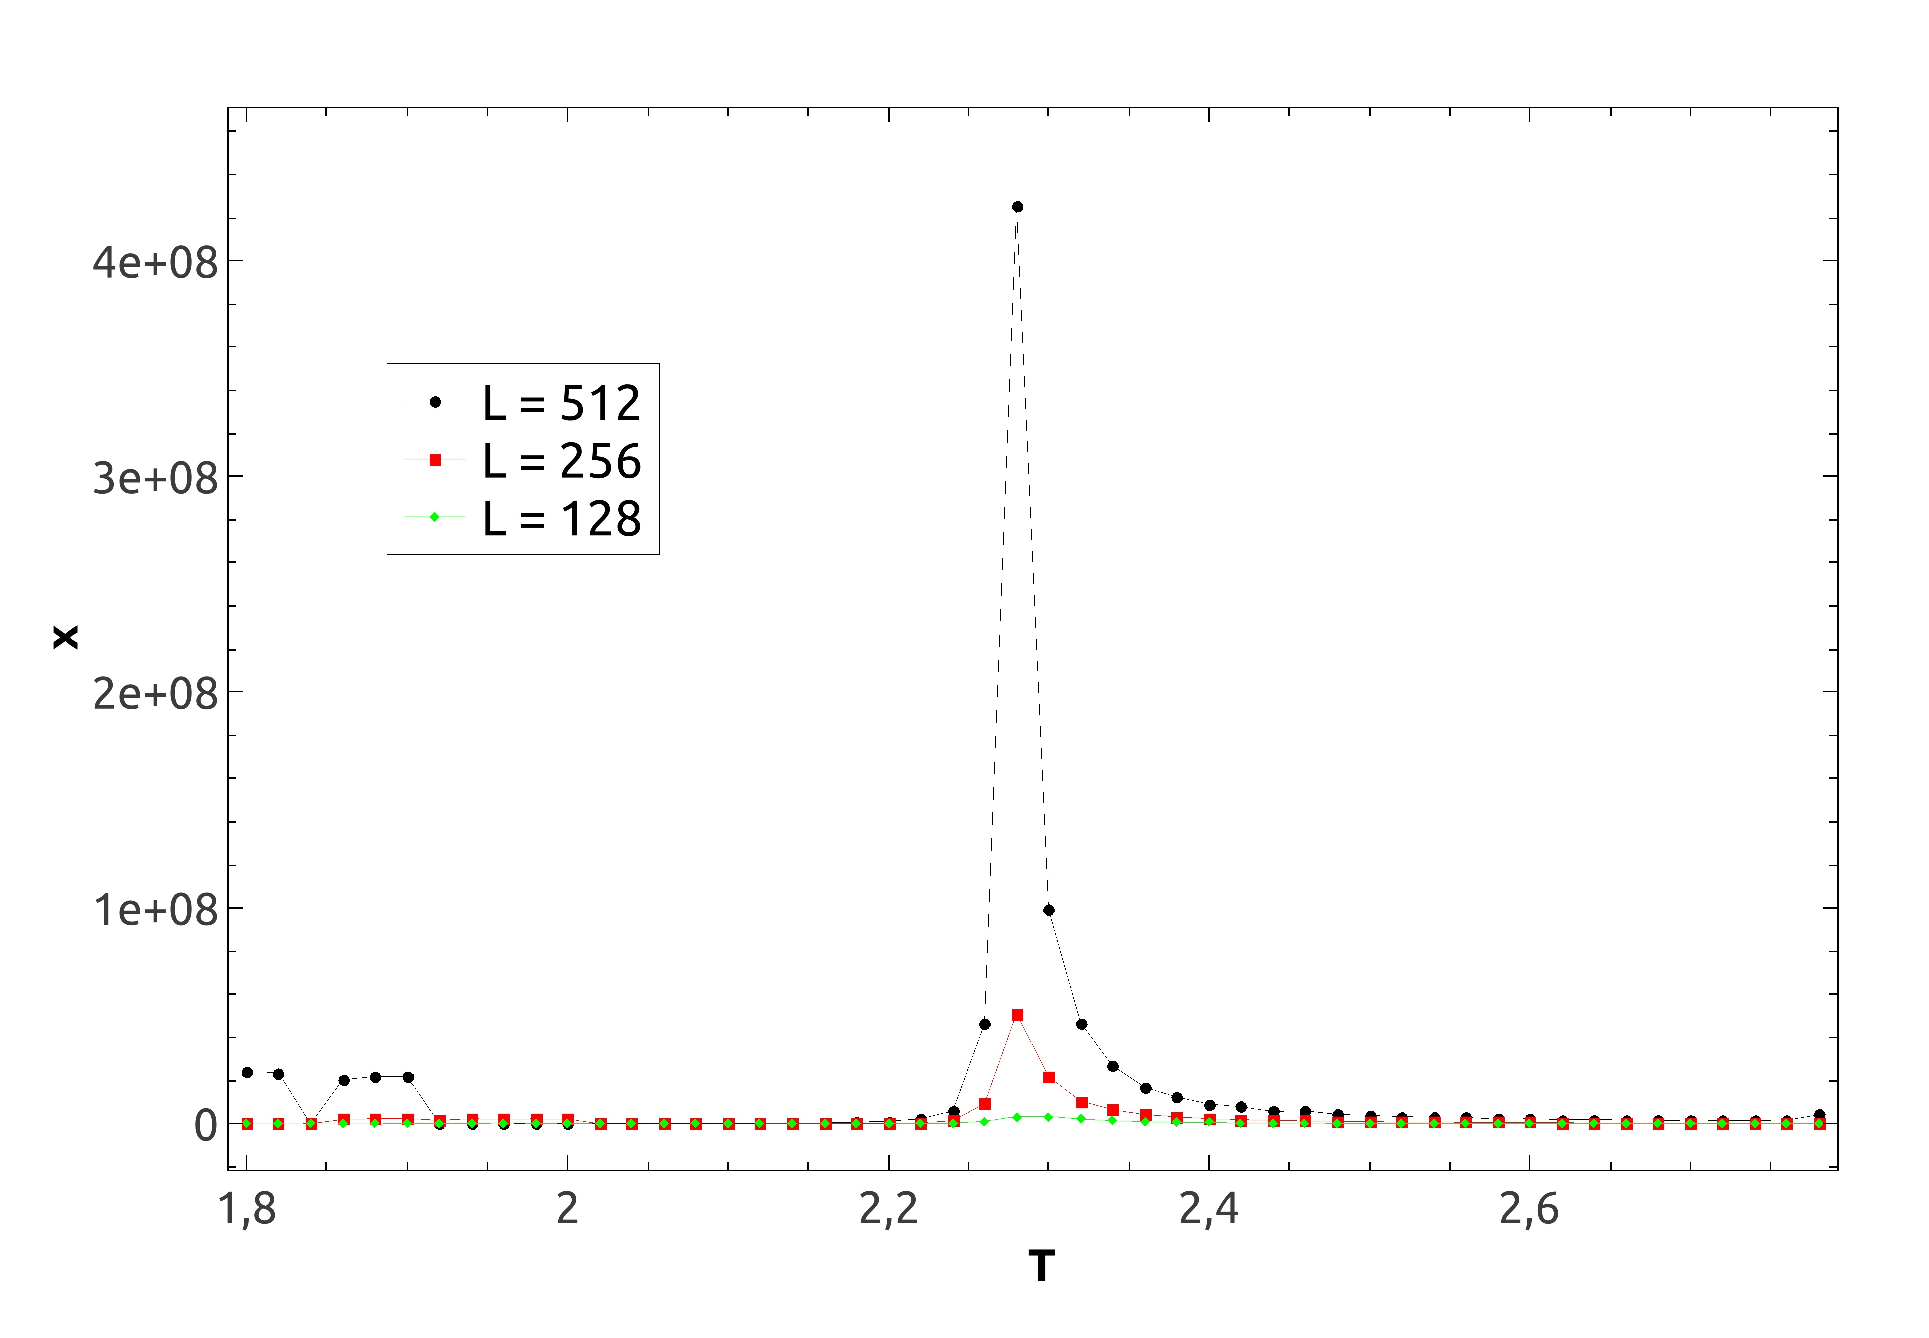
\includegraphics[scale=0.4]{chi}
	}
	\end{center} 
Так же на интервале $T \in[1.8, 1.9]$ можно заметить скачек восприимчивости, его природа еще не определена. Будут проведены дополнительные исследования этой области.
	\section{Поиск критической температуры}
	Кумулянта Биндера определятся как $U = \frac{1}{2}(3 - \frac{<M^4>}{{<M^2>}^2})$, так же нам известно, что $U \sim (T - T_C)$, это означает , что кумулянта систем с разными размерами будет иметь точку пересечения в $T_C$, но так как рассчитанная кумулянта имеет погрешность, вместо точки мы получим треугольник, центр тяжести которого мы выберем в качестве $T_C$. 
	В результате моделирования были получены результаты , представленные на графике ниже
	\begin{center}
		\mbox{
			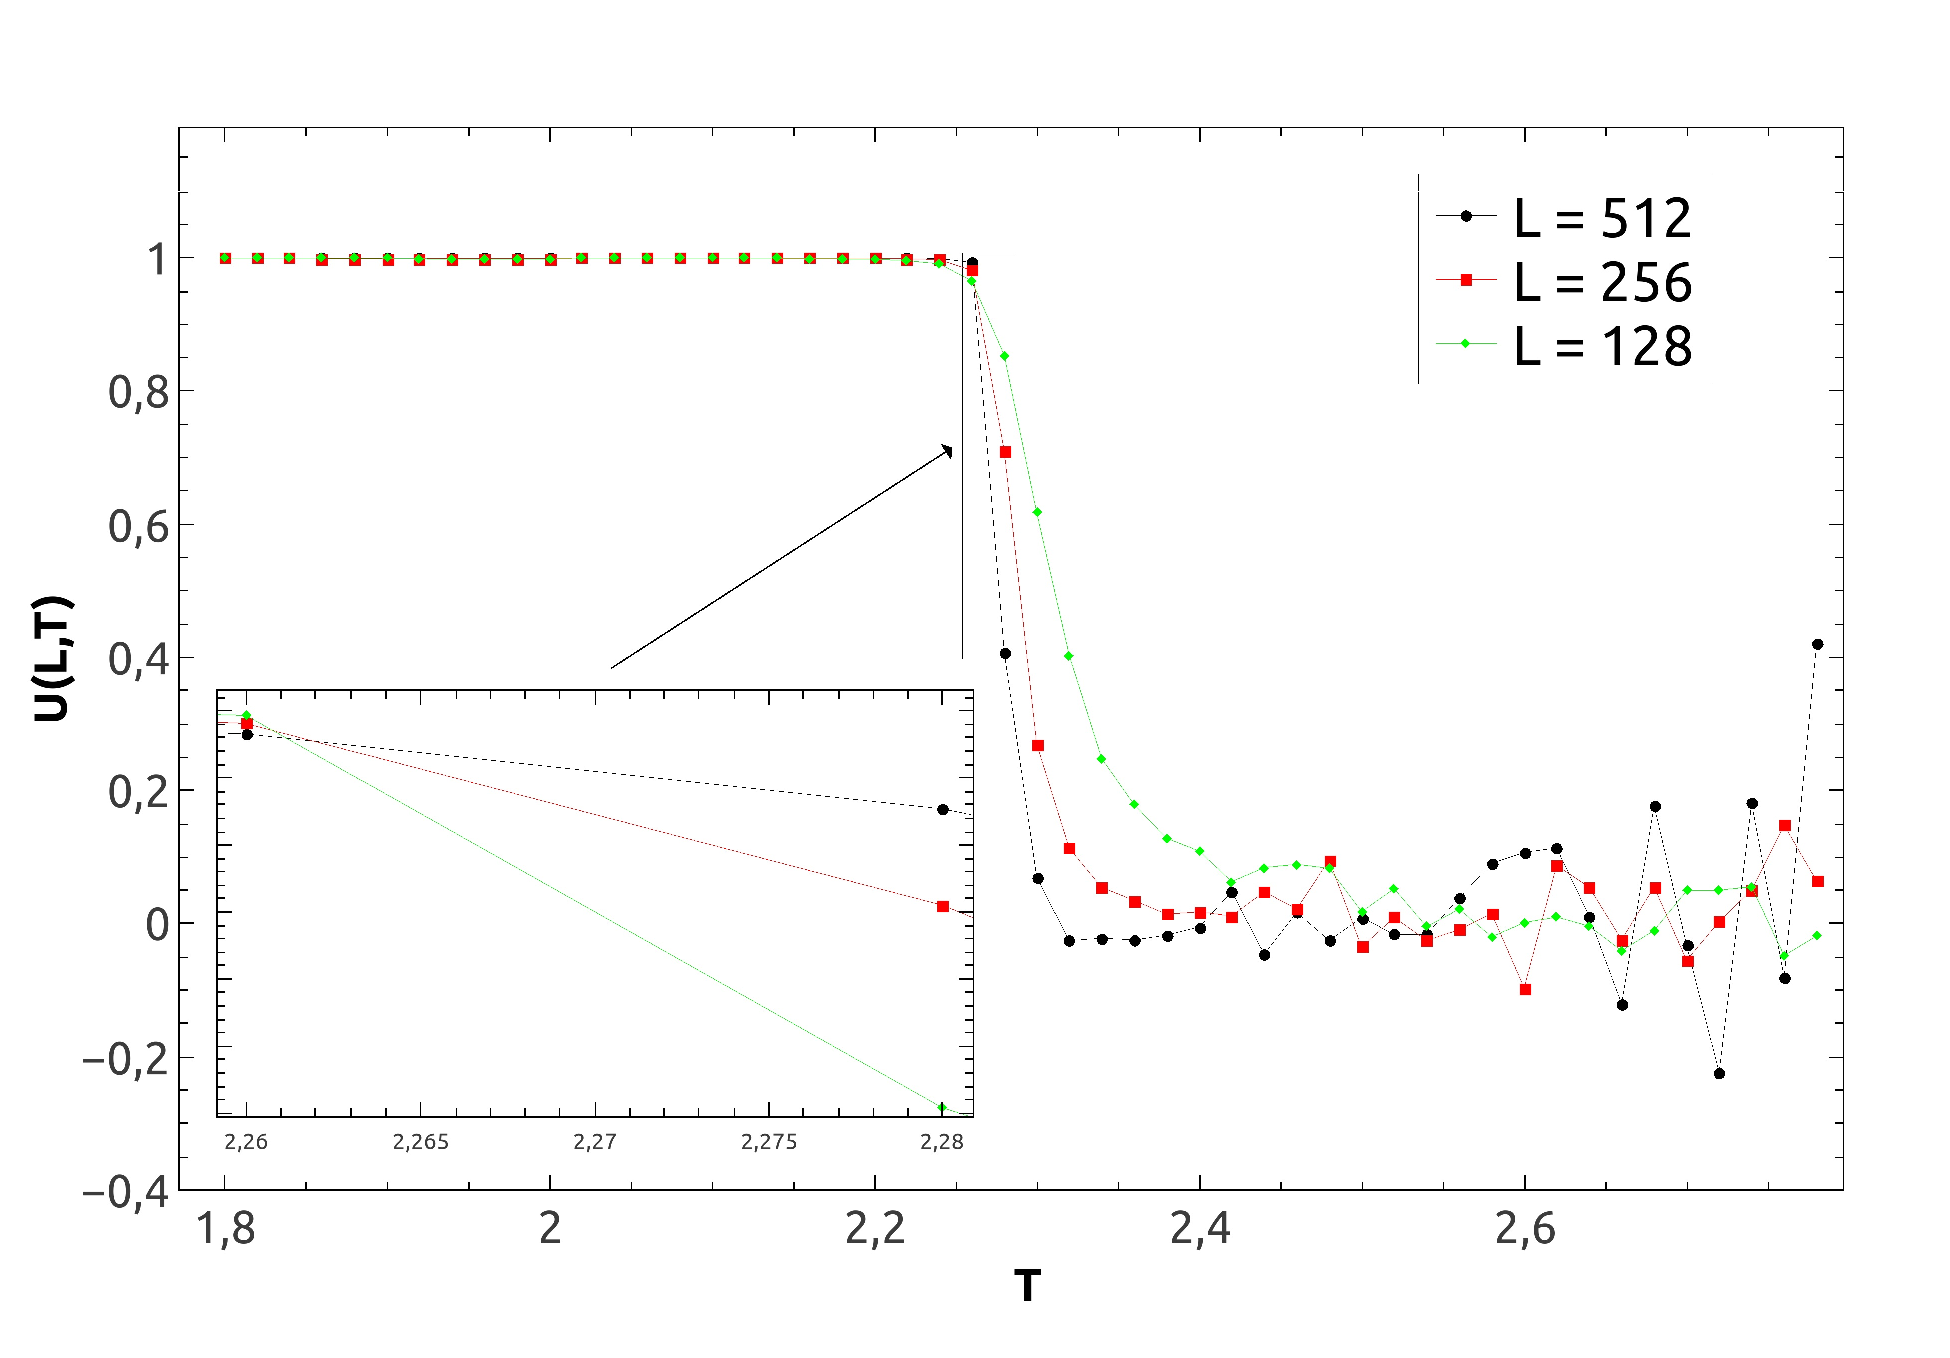
\includegraphics[scale=0.4]{U(L,T)}
		}
	\end{center} 
	Следующий интервал для исследования $- T \in[2.26, 2.28]$. Исходя из ранее полученного опыта и результатов, можно предположить, что после изучения этого интервала $T_C$ будет получена с точностью $\sim {10}^{-5}$.
	\section{Исследование времени расчетов}
	\begin{center}
		\begin{tabular}{|c|c|c|c|}
			\hline
			\multicolumn{4}{|c|}{L}\\
			\hline
			Модель процессора
			& ryzen 3 1200
			& Аналитическое
			& Модуль разницы \\
			\hline
			Мат. ожидание& 0.499988 & 0.5 & 0.000012 \\
			\hline
			Дисперсия& 0.0833343 & 0.8333333 & 0.000001 \\
			\hline
			Ассиметрия& 0.000204552 & 0 & 0.000204552 \\
			\hline
			Эксцесс& -1.20006 & -1.2 & 0.00006 \\
			\hline
			\hline
		\end{tabular}
	\end{center}
	
%>>>>>>>>>>>>>>>>>>>>>>>>>>>>>>>>>>>>>>>>>>>>>>>>>>>>

\newpage
\end{document}
